\subsection{Validation}
\label{sec:validation}
%\begin{figure}[t]
%	\centering
%	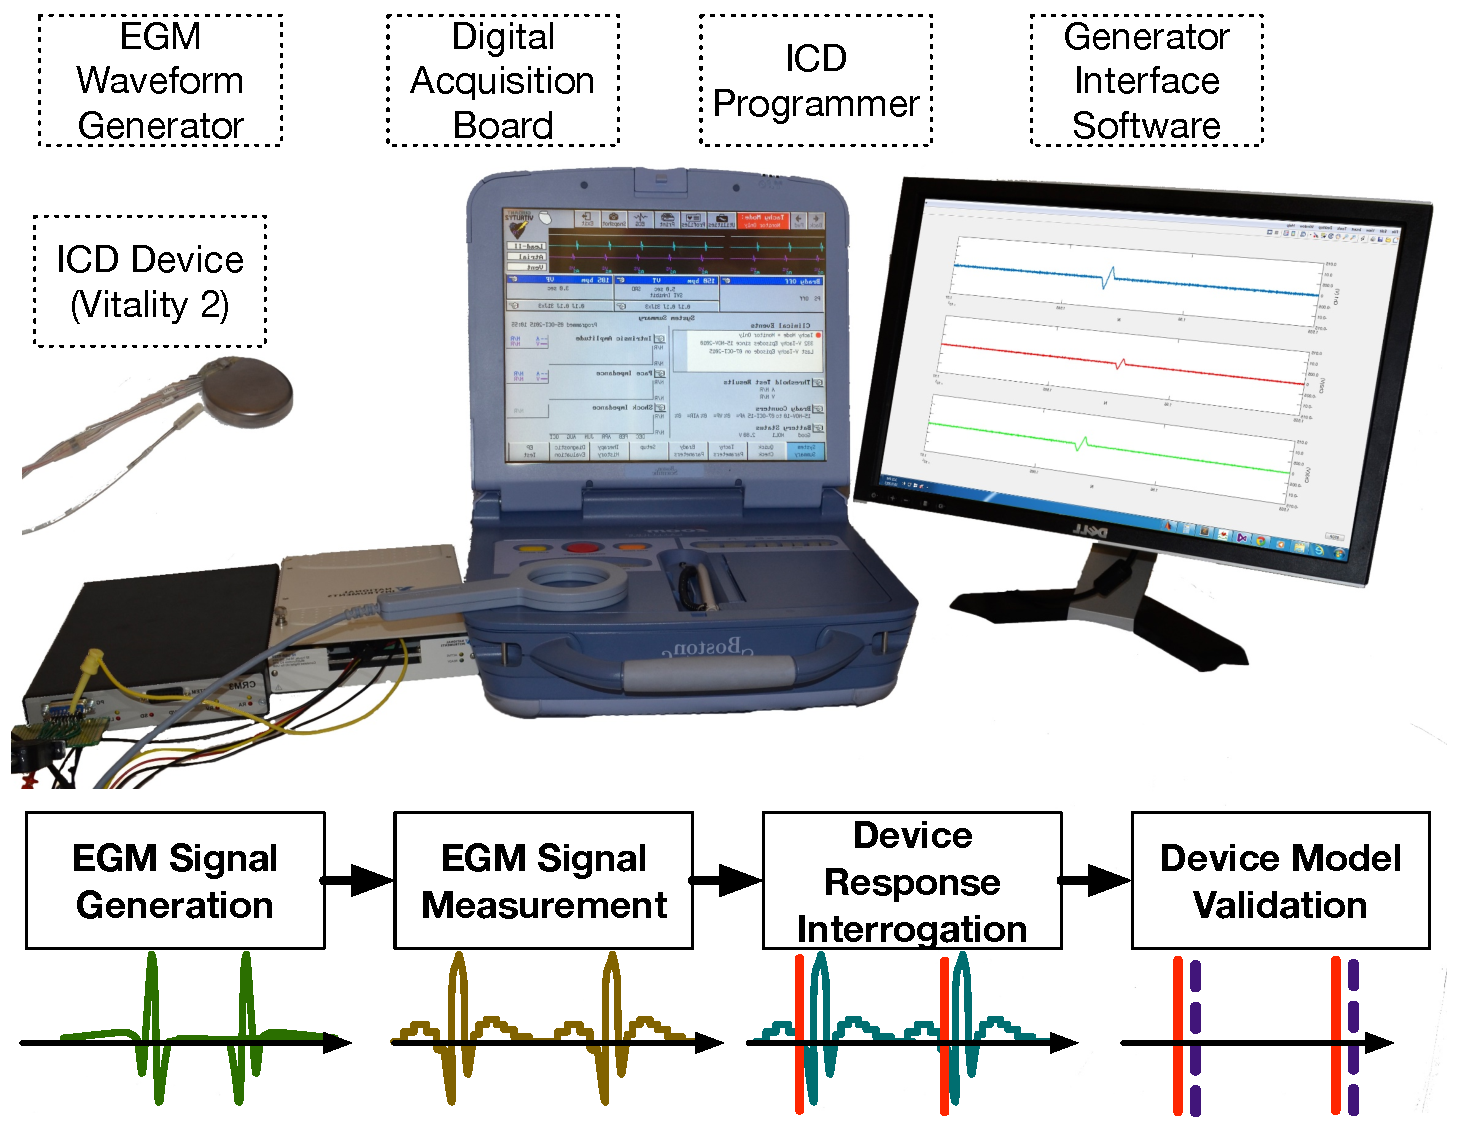
\includegraphics[scale=0.28]{figures/figValidationSetup.pdf}
%	\vspace{-10pt}
%	\caption{\small Model Validation. 14 different scenarios were generated from the EGM waveform generator for Boston Scientific and input into the Vitality 2 ICD. The input signal was acquired through the DAQ board and applied to the device model implementation. The ICD response was interrogated using the ICD programmer and compared to the output of the device model.}
%	\vspace{-10pt}
%	\label{fig:validationSetup}
%\end{figure}
\mynote{SD}{What about Medtronic. As I have mentioned previously, whenever you provide details of one vendors algorithm, you have to do the same for the other vendor. Otherwise the comparison seems biased towards one versus the other.}
\begin{figure}[t ]
	\centering
	\includegraphics[scale=0.28]{figures/figScreenshot.pdf}
	\caption{\small Example of validation output screenshots (Ventricular fibrillation) showing matching therapy decision for the ICD and our implementation.}
	\vspace{-10pt}
	\label{fig:validation}
\end{figure}

Conformance testing was used to validate the software implementations of the Vitality II device by Boston Scientific. 
The validation hardware setup is illustrated in Fig.~\ref{fig:validation}. 
14 different scenarios were specified and programmed into an EGM Waveform generator (CRM3 Simulator, Guidant, USA) such that it would output a signal to the connected Vitality II device.
The various scenarios traverse 7 out of 9 branches of the detection algorithm for Boston Scientific described in Sec. \ref{sec:svtvt} and shown in Fig. \ref{fig:BS_det}. 
The response of the \ac{ICD} interrogated using an ICD programmer (ZOOM Latitiude, Boston Scientific).
As the waveform was applied to the ICD, the waveform was simultaneously acquired using a National Instruments \ac{DAQ} board.
The recorded waveform was then applied to the device model and response was compared.
Fig. \ref{fig:validation} shows an example of one such scenario, specificallly \ac{VF}. 
In this case, the software model matched to the decision of the actual \ac{ICD} which also determined that therapy should be applied.

In all scenarios, the decision of model conformed to that of the \ac{ICD}. 
The remaining two branches were not reachable due to the limited output capability of the programmer.
The Medtronic software implementation can be validated using a similar process.
